\chapter{Programs and Expressions}

This chapter presents many of the key features of Unicon, starting
with those it has in common with other popular languages. Detailed
instructions show how to \index{compile}compile and \index{run}run
programs. Soon the examples introduce important ways in which Unicon
is different from other languages. These differences are more than
skin deep. If you dig deeply, you can find dozens of details where
Unicon provides just the right blend of simplicity, flexibility, and
power.  After this chapter, you will know how to
\begin{itemize}\itemsep0pt
  \item edit, compile, and execute Unicon programs
  \item use the basic types to perform calculations
  \item identify expressions that can \index{expression failure}fail, or
    produce multiple results
  \item control the flow of execution using conditionals, looping, and
    procedures
\end{itemize}

\section{Your First Unicon Program}

This section presents the nuts and bolts of writing and running an
Unicon program, after which you will be able to try
the code examples or write your own programs. Before you can run the
examples here or in any subsequent chapter, you must
\index{install}install Unicon on your system. (See Appendix F for
details on downloading and installing Unicon from the Unicon web site,
http://unicon.org.) We are going to be very explicit here,
and assume nothing about your background. If you are an experienced
programmer, you will want to skim this section, and move on to the next
section. If you are completely new to programming, have no fear. Unicon
is pretty easy to learn.

All programs consist of commands that use hardware to obtain or present
information to users, and perform calculations that transform
information into a more useful form. To program a
computer you write a document containing instructions for the computer
to carry out. In Unicon a list of instructions is called
a \index{procedure}\textit{procedure}, and a
\index{program}\textit{program} is a collection of one or more
procedures. In larger programs, groups of related procedures are
organized into classes or packages; these features are presented in
Part II of this book. Unicon programs are text files that may be
composed using any text \index{editor}editor. For the purposes of
demonstration this section describes how to use \index{Ui}Ui, the
program editor and integrated development tool that comes with Unicon.

It is time to begin. Fire up Ui by typing
"ui" from the command line, or launching
the menu item or icon labeled "Unicon," and
type:

\iconcode{
procedure main() \\
\>   write("Hello, amigo!") \\
end
}

Your \index{screen}screen should look something like Figure 1-1. The
large upper area of the window is the editing region where you type
your program code. The lower area of the window is a status region in
which the Ui program displays a message when a command completes
successfully, or when your program has an error. Until you explicitly
name your file something else, a new file has the name
\textsf{noname.icn}. The font Ui uses to display
\index{source code}source code is selectable from the Options menu.

\begin{center}
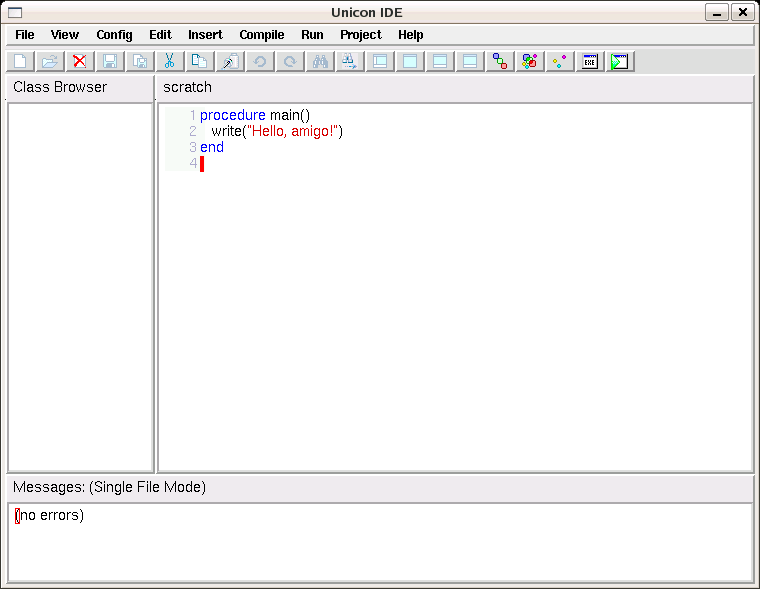
\includegraphics[width=6in,height=4.5953in]{ub-img/ub-img5.png}
\end{center}
\vspace{-0.25cm}{\sffamily\bfseries Figure 1-1:}
{\sffamily Writing an Unicon program using the Ui program.}

\bigskip

The list of instructions that form a \textit{procedure} begins with
the word \texttt{procedure} and ends with the word
\texttt{end}. Procedures have names. After writing a list of
instructions in a procedure you may refer to it by name without
writing out the list again. The \texttt{write()} instruction is just
such a procedure, only it is already written for you; it is built in
to the language. When you issue a \texttt{write()} instruction, you
tell the computer what to write. The details a procedure uses in
carrying out its instructions are given inside the parentheses
following that procedure's name; in this case, \texttt{"Hello, amigo!"}
is to be written.  When you see parentheses after a name in
the middle of a list of instructions, it is an instruction to go
execute that procedure's instructions. Inside the parentheses there
may be zero, one, or many values supplied to that procedure.

Besides writing your program, there are a lot of menu commands that you can use
to control the details of compiling and executing your program within Ui. For
instance, if you select \textbf{Run$\to$Run}, Ui will do the following
things for you.
\begin{enumerate}
  \item Save the program in a file on disk\texttt{.}  All Unicon programs end
    in \texttt{.icn}; you could name it anything you wished, using the
    \textbf{File$\to$SaveAs} command.
  \item Compile the Unicon program from human-readable text to (virtual)
    machine language. To do this step manually, you can select the
    \textbf{Compile$\to$Make executable} command.
  \item Execute the program. This is the main purpose of the \textbf{Run}
    command. Ui performed the other steps in order to make this operation
    possible.
\end{enumerate}
If you type the \texttt{hello.icn} file correctly, the computer should
chug and grind its teeth for awhile, and

\iconcode{
\>   Hello, amigo!
}

\noindent should appear in a window on your screen. This ought to be pretty
intuitive, since the instructions included the line

\iconcode{
\>   write("Hello, amigo!")
}

\noindent in it. That's how to write to the screen.
It's that simple.

The first procedure to be executed when a program runs is called
\texttt{main()}. Every instruction listed in the procedure named
\texttt{main()} is executed in order, from top to bottom, after which
the program terminates. Use the editor to add the following lines right
after the line \texttt{write("Hello,
amigo")} in the previous program:

\iconcode{
\>   write("How are you?") \\
\>   write(7 + 12)
}

\noindent The end result after making your changes should look like this:

\iconcode{
procedure main() \\
\>   write("Hello, amigo!") \\
\>   write("How are you?") \\
\>   write(7 + 12) \\
end
}

Run the program again. This example shows you what a list of
instructions looks like, as well as how easy it is to tell the computer
to do some arithmetic.

{\sffamily\bfseries
Note}

{\sffamily
It would be fine (but not very useful) to tell the computer to add 7 and
12 without telling it to write the resulting value. On seeing the
instruction}

\iconcode{
\>   7 + 12
}

\noindent
the computer would do the addition, throw the 19 away, and go on.

Add the following line, and run it:

\iconcode{
\>   write("7 + 12")
}

This illustrates what quotes are for. Quoted text is taken
literally; without quotes, the computer tries to simplify (do
some arithmetic, or compute the value of what is written), which might
be difficult if the material in question is not an expression!

\iconcode{
\>   write(hey you)
}

\noindent makes no sense and is an error. Add this line, and run it:

\iconcode{
\>   write(7 + "12")
}

The 12 in quotes is taken literally as some text, but that text happens
to be digits that comprise a number, so adding it to another number
makes perfect sense. The computer will not have as much success if you
ask it to add 7 to {\textquotedblleft}amigo{\textquotedblright}. The
computer views all of this in terms of values. A \textit{value} is a
unit of information, such as a number. Anything enclosed in quotes is a
single value. The procedure named \index{write()}\texttt{write()}
prints values on your screen. \textit{Operators} such as \texttt{+}
take values and combine them to produce other values, if it is possible
to do so. The values you give to \texttt{+} had better be numbers! If
you try to add something that doesn't make sense, the
program will stop running at that point, and print an error message.

By now you must have the impression that writing things on your screen
is pretty easy. Reading the \index{keyboard}keyboard is just as easy,
as illustrated by the following program:

\iconcode{
procedure main() \\
\>   write("Type a line ending with
		{\textless}ENTER{\textgreater}:") \\
\>   write("The line you typed was" , read()) \\
end
}

Run the program to see what it does. The procedure named
\index{read()}\texttt{read()} is used to get what the user types. It is
built in to the language. The \texttt{read()} instruction needs no
directions to do its business, so nothing is inside the parentheses.
When the program is run, \texttt{read()} grabs a line from the
keyboard, turns it into a value, and produces that value for use in the
program, in this case for the enclosing \texttt{write()} instruction.

\texttt{The }\texttt{write()} instruction is happy to print out more
than one value on a line, separated by commas. When you run the
program, the \texttt{"the line you typed
was"} part does not get printed until after you type the
line for \texttt{read()} and that instruction completes. The
\texttt{write()} instruction must have all of its directions (the
values inside the parentheses) before it can go about its business.

Now let's try some variations. Can you guess what the
following line will print?

\iconcode{
\>   write("this line says " ,
"read()")
}

The \texttt{read()} procedure is never executed because it is quoted!
Quotes say "take these letters literally, not
as an equation or instruction to evaluate." How about:

\iconcode{
\>   write("this line says , read()")
}

\noindent Here the quotes enclose one big value, which is printed, comma
and all. The directions one gives to a procedure are
\textit{parameters}; when you give a procedure more than one parameter,
separated by commas, you are giving it a
\index{parameter list}\textit{parameter list}. For example,

\iconcode{
\>   write("this value ",
"and this one")
}

\noindent Compile and run the following strange-looking program.
What do you think it does?

\iconcode{
procedure main() \\
\>   while write( "" \~{}== read() ) \\
end
}

This program copies the lines you type until you type an empty line by
pressing Enter without typing any characters first. The
\texttt{""} are used just as usual. They
direct the program to take whatever is quoted literally, and this time
it means literally nothing - an empty line. The operator
\texttt{\~{}==} stands for "\index{not equals}not
equals". It compares the value on its left to the value
on its right, and if they are not equal, it produces the value on the
right side; if they are equal, it \index{expression
failure}\textit{fails} - that is, the {\textquotedblleft}not
equals{\textquotedblright} operator produces no value. If you have
programmed in other languages, this may seem like a strange way to
describe what is usually performed with nice simple Boolean values True
and False. For now, try to take this description at face value; Unicon
has no Boolean type or integer equivalent, it uses a more powerful
concept that we will examine more fully in the chapters that follow.

Thus, the whole expression \texttt{"" \~{}==
read()} takes a line from the keyboard, and if it is not empty, it
produces that value for the enclosing \texttt{write()} instruction.
When you type an empty line, the value \texttt{read()} produces is
equal to \texttt{""}, and \texttt{\~{}==}
produces no value for the enclosing \texttt{write()} instruction, which
similarly fails when given no value. The \index{while}\texttt{while}
instruction is a "\index{loop}loop" that
repeats the instruction that follows it until that instruction fails
(in this case, until there is no more input). There are other kinds of
loops, as well as another way to use \texttt{while}; they are all
described later in this chapter.

So far we've painted you a picture of the Unicon
language in very broad strokes, and informally introduced several
relevant programming concepts along the way. These concepts are
presented more thoroughly and in their proper contexts in the next
sections and subsequent chapters. Hopefully you are already on your way
to becoming an Icon programmer \textit{extraordinaire}. Now it is time
to dive into many of the nuts and bolts that make programming in Unicon
a unique experience.

\section{Command Line Options}

Unicon comes with an IDE, but you can edit programs with any
editor, and compile and run them from your operating
system's command line. This section describes the
Unicon command line tools along with several useful options. The Unicon
compiler executable is named unicon, and to compile the program foo.icn
you would type

\iconcode{
\>   unicon foo
}

\noindent To execute the resulting program, just type

\iconcode{
\>   foo
}

To compile and link a program consisting of several modules, you can
type them all on the command line, as in

\iconcode{
\>   unicon foo bar baz
}

\noindent but often you will want to compile them separately
(using the -c command line option) and link the resulting object
files, called ucode files; their extension is .u

\iconcode{
\>   unicon -c foo\newline \\
\>   unicon -c bar\newline \\
\>   unicon -c baz\newline \\
\>   unicon foo.u bar.u baz.u
}

Some of the other useful command line options include:

\begin{itemize}
\item \texttt{{}-o arg}\ \ \ \ name the resulting output file arg
\item \texttt{{}-x args}\ \ execute the program immediately after linking;
		 this option goes \textit{after} the program filenames
\item \texttt{{}-t}\ \ \ \ turn on tracing
\item \texttt{{}-u}\ \ \ \ produce a warning for undeclared variables
\end{itemize}

These options can be specified in the Ui program under the Compile
menu's Compile Options command. Other options exist;
consult your Unicon and Icon manual pages and platform-specific help
files and release information for more details.

\section{Expressions and Types}

Each \index{procedure}procedure in a Unicon program is a sequence of
\index{expression}\textit{expression}\textit{s.} Expressions are
instructions for obtaining \index{value}values of some
\index{type}type, such as a number or a word; some expressions also
cause side effects, such as sending data to a hardware device.
Simple expressions just read or write a value stored in
memory. More interesting expressions specify a computation that
manipulates zero or more \index{argument}\textit{argument} values to
obtain \index{result}\textit{result} values by some combination of
operators, procedures, or \index{control structure}control structures.

The simplest expressions are \index{literal}\textit{literal}\textit{s},
such as \texttt{2} or \texttt{"hello,
world!"}\texttt{. }These expressions directly specify a
value stored in memory. When the program runs, they do not do any
computation, but rather evaluate to themselves. Literals are combined
with other values to produce interesting results. Each literal has a
corresponding \textit{type}. This chapter focuses on the \index{atomic
types}atomic types. Atomic types represent individual, \index{immutable
values}immutable values. The atomic types in Unicon are
\index{integer}integer and \index{real number}real (floating-point)
numbers, \index{string}string (a sequence of characters), and
\index{cset}cset (a \index{character set}character set). Atomic types
are distinguished by the fact that they have literal values, specified
directly in the program code and represented as data in the compiled
code. Values of other types such as lists are constructed during
execution. Later chapters describe structure types that organize
collections of values, and system types for interacting with the
operating system via files, databases, windows, and network
connections. 

After literals, \index{reference}references to
\index{variable}\textit{variable}\textit{s} are the next simplest form
of expression. Variables are named memory locations that hold values
for use in subsequent expressions. You refer to a variable by its name,
which must start with a letter or underscore and may contain any number
of letters, underscores, or numbers. Use names that make the meaning of
the program clear. The values stored in variables are manipulated by
using variable names in expressions like \texttt{i+j}. This expression
results in a value that is the sum of the values in the variables
\texttt{i} and \texttt{j}, just like you would expect.

Some words may not be used as variable names because they have a special
meaning in the language. These \index{reserved word}\textit{reserved
words} include \texttt{procedure}, \texttt{end},
\texttt{while}, and so on. Other special variables called
\index{keyword}\textit{keywords} start with the ampersand
character (\texttt{\&}) and denote special values. For example, global
variables are initialized to the null value represented by the keyword
\texttt{\&null}\index{null value, \&null}. Other keywords
include \texttt{\&date}, \texttt{\&time}, and so on.
Complete lists of reserved words and keywords are given in Appendix A.

Unlike many languages where you have to state up front
(\textit{declare}) all the variables you are going to use\textit{ }and
specify their data type, in Unicon variables do not have to be declared
at all, and any variable can hold any type of value. However, Unicon
will not allow you to mix incompatible types in an expression. Unicon
is \index{type safe}\textit{type safe}, meaning that every operator
checks its argument values to make sure they are compatible, converts
them if necessary, and halts execution if they cannot be converted.

\section{Numeric Computation}

Unicon supports the usual \index{arithmetic}arithmetic operators on
data types \index{integer}integer and real. Integers are
signed whole numbers of arbitrary magnitude. The real type is a signed
\index{floating point}floating point decimal number whose size on any
platform is the largest size supported by machine instructions,
typically 64-bit double precision values. In addition to
\index{addition}addition (\texttt{+}), \index{subtraction}subtraction
(\texttt{{}-}), \index{multiplication}multiplication (\texttt{*}) and
\index{division}division (\texttt{/}), there are operators for
\index{modulo \%}modulo (\texttt{\%}) and \index{exponentiation
\^{}}exponentiation (\texttt{\^{}}). Arithmetic operators require
numeric operands.

{\sffamily\bfseries
Note}

{\sffamily
Operations on integers produce integers; fractions are truncated, so 8/3
produces 2. If either operand is a real, the other is converted to real
and the result is real, so 8.0/3 is 2.66666...}

As a general rule in Unicon, arguments to numeric operators and
functions are automatically \index{type conversion!type
conversion}converted to numbers if possible, and a \index{run-time
error}run-time error occurs otherwise. The built-in functions
\index{integer(x)}\texttt{integer(x)} and
\index{real(x)}\texttt{real(x)} provide an explicit conversion
mechanism that fails if \texttt{x} cannot be converted to numeric
value, allowing a program to check values without resulting in a
run-time error.

In addition to the operators, built-in functions support several common
\index{numeric operations}numeric operations. The
\index{sqrt(x)}\texttt{sqrt(x)} function produces the square root of x,
and \index{exp(x)}\texttt{exp(x)} raises \textit{e} to the \texttt{x}
power. The value of \index{pi, 3.14... \&pi}\textit{pi} (3.141...) is
available in keyword \texttt{\&pi}, the \index{golden ratio 1.618...,
\&phi}Golden Ratio (1.618...) is available in \index{phi 1.618...,
\&phi}\texttt{\&phi}, and \textit{e} (2.718...) is available in
\index{e, 2.71... \&e}\texttt{\&e}. The \index{log(x)}\texttt{log(x)}
function produces the \index{natural log, log(x)}natural log of
\texttt{x}. The common \index{trigonometric function}trigonometric
functions, such as \index{sin()}\texttt{sin()} and
\index{cos()}\texttt{cos()}\texttt{ }take their angle arguments in
\index{radian}radian units. The \index{min()}\texttt{min(x1, x2, ...)}
and \index{max()}\texttt{max(x1, x2, ...)} routines return minimum and
maximum values from any number of arguments. Appendix A gives a
complete list of built-in functions and operators.

Listing 1-1 shows a simple Unicon program that illustrates the use of
variables in a numeric computation. The line at the beginning is a
comment for the human reader. \index{comment}Comments begin with the
\texttt{\#} character and extend to the end of the line on which they
appear. The compiler ignores them.

\bigskip

{\sffamily\bfseries Listing 1-1}
{\sffamily\bfseries Mystery program}

\iconcode{
\# What do I compute? \\
procedure main() \\
\>   local i, j, old\_r, r \\
\>   i := read() \\
\>   j := read() \\
\>   old\_r := r := min(i, j) \\
\>   while r {\textgreater} 0 do \{ \\
\>\>    old\_r := r \\
\>\>    if i {\textgreater} j then \\
\>\>\>     i := r := i \% j \\
\>\>    else \\
\>\>\>     j := r := j \% i \\
\>\>    \} \\
\>   write(old\_r) \\
end
}

This example illustrates \index{assignment}\textit{assignment}; values
are assigned to (or "stored in") variables
with the \texttt{:=} operator. As you saw in the previous section, the
function \texttt{read()} reads a line from the input and returns its
value. The modulo operator (\texttt{\%}) is an important part of this
program: \texttt{i \% j} is the \index{remainder}remainder when
\texttt{i} is divided by \texttt{j}.

While \index{loop}loops can use a reserved word
\texttt{do} followed by an expression (often a compound expression
in curly braces). The expression following the \texttt{do} is
executed once each time the expression that controls the \texttt{while}
succeeds. Inside the \texttt{while} loop, a
\index{conditional expression}conditional
\index{if-then-else}\texttt{if-then-else} expression is used to select
from two possible actions.

The names of the variables in this example are obscure, and there are no
comments in it other than the one at the top. Can you guess what this
program does, without running it? If you give up, try running it with a
few pairs of positive numbers.

In addition to arithmetic operators, there are \index{augmented
assignment}\textit{augmented assignment} operators. To
increment the value in a variable by 2, these two statements are
equivalent:

\iconcode{
\>   i +:= 2 \\
\>   i := i + 2
}

Augmented assignment works for most \index{binary operator}binary
operators, not just arithmetic. The expression \texttt{i
}\texttt{\textit{op}}\texttt{:= expr} means the same as \texttt{i := i
}\texttt{\textit{op}}\texttt{ expr}.

\section{Strings and Csets}

The non-numeric atomic types in Unicon are character sequences
(\index{string}strings) and \index{character set}character sets
(\index{cset}csets). Icon came from the domain of string
processing, and from it Unicon inherits many sophisticated features for
manipulating strings and performing \index{pattern matching}pattern
matching. This section presents the simple and most common operations.
More advanced operations and examples using strings and csets are given
in Chapter 4.

\index{string!literal}String literals are enclosed in double quotes, as
in \texttt{"this is a string"}, while
\index{cset literal}cset literals are enclosed in single quotes, as in
\texttt{'aeiou'}. Although strings
and csets are composed of characters, there is no
\index{character}character type; a string (or cset) consisting of a
single character is used instead.

Current implementations of Unicon use eight-bit characters, allowing
strings and csets to be composed from 256 unique characters.
\index{ASCII}ASCII representation is used for the lower 128 characters,
except on \index{EBCDIC}EBCDIC systems. The appearance of non-ASCII
values is platform dependent. Like integers, strings can be arbitrarily
large, constrained only by the amount of memory you have on your
system.

Several operators take string arguments. The \index{string!length
(*s)}\texttt{*s} operator gives the \index{length operator (*x)}length
of string \texttt{s}. The expression \index{string!concatenation s1
{\textbar}{\textbar} s2}\texttt{s1{\textbar}{\textbar}s2} produces a
string consisting of the characters in \texttt{s1} followed by
\texttt{s2}. The \index{subscript operator}subscript operator
\index{string!subscript (s[i])}\texttt{s[i]} produces a one-letter
substring of \texttt{s} at the \texttt{i}th position.
\index{string!indexes 1-based}Indices are counted starting from
position 1. If \texttt{i} is nonpositive, it is from the end of the
string, for example \texttt{s[-2]} is the second to the last character
in the string.

Csets support set operators. \index{union (c1 ++ c2)}\texttt{c1++c2}
produces a cset that is the union of \texttt{c1} and \texttt{c2}.
The expression \index{intersection (c1**c2)}\texttt{c1**c2} is the
intersection, while \index{difference (c1 -{}- c2)}\texttt{c1-{}-c2} is
the difference. In addition, several keywords are commonly used
csets. The keywords \index{letters,  \&letters}\texttt{\&letters},
\texttt{\&lcase}, and \texttt{\&ucase} denote the alphabetic
characters, \index{lower case}lower case characters a-z, and
\index{upper case}upper case characters A-Z, respectively, while
\index{digits, \&digits}\texttt{\&digits} is the set from 0-9,
\index{ASCII, \&ascii}\texttt{\&ascii} is the lower 128 characters, and
\index{cset, universal \&cset}\texttt{\&cset} is the set of all (256,
on most implementations) characters.

Many built-in functions operate on strings and csets. Some of the simple
string functions are \index{reverse(x)}\texttt{reverse(s)}, which
produces a string that is the reverse of \texttt{s}, and
\index{trim(s,c)}\texttt{trim(s,c)}, which produces a substring of
\texttt{s} that does not end with any character in cset \texttt{c}.

Functions and operators that require string arguments convert numeric
values to strings automatically, and halt execution with a run-time
error if given a value that cannot be converted to a string.

\section{Goal-directed Evaluation}

\index{goal-directed evaluation}So far, the examples of how
expressions are evaluated have included nothing you
wouldn't find in ordinary programming languages. It is
time to push past the ordinary.
In most conventional languages, each expression always computes
\textit{exactly one} result. If no valid result is possible, a
\index{sentinel value}sentinel value such as -1, NULL, EOF
(\index{end-of-file}end-of-file) or INF (\index{infinity}infinity) is
returned instead. This means that the program must check the return
value for this condition. For example, while reading integers from the
input and performing some operation on them you might do something like
this:

\iconcode{
\>   while (i := read()) \~{}= -1 do \\
\>\>     process(i)
}

This will work, of course, except when you really need to use -1 as a
value! It is somewhat cumbersome, however, even when a sentinel value
is not a problem. Unicon provides a much nicer way to write this type
of code, developed originally in the Icon language. In Unicon,
expressions are \textit{goal-directed}. This means that every
expression when evaluated has a goal of producing results for the
surrounding expression. If an expression succeeds in producing a
result, the surrounding expression executes as intended, but if an
expression cannot produce a result, it is said to \index{expression
failure}fail and the surrounding expression cannot be performed and in
turn fails.

Now take a look at that loop again. If it weren't for
the termination condition, you would not need the
intermediate variable \texttt{i}. If you would like to say:

\iconcode{
\>   process(read())
}

\noindent
your wishes are answered by Unicon; you can indeed write your
program like this. The expression \texttt{read()} tries to produce a
value by reading the input. When it is successful, \texttt{process()}
is called with the value; but when \texttt{read()} cannot get any more
values, that is, at the end of the file, it \textit{fails}. This
failure propagates to the surrounding expression and \texttt{process()}
is not called either. Here is the clincher: control expressions like
\texttt{if} and \texttt{while} don't check for Boolean
(true/false) values, they check for \index{success}success! So our loop
becomes

\iconcode{
\>   while process(read())
}

The \index{do clause}\texttt{do} clause of a \texttt{while} loop is
optional; in this case, the \index{condition}condition does everything
we need, and no \texttt{do} clause is necessary.

Consider the \index{if statement}\texttt{if}\texttt{ }statement that was
used in the earlier arithmetic example:

\iconcode{
\>   if i {\textgreater} j then ...
}

Comparison operators such as \texttt{{\textgreater}} succeed or fail
depending on the values of the operands. This leads to another
question: if an expression like \texttt{i {\textless} 3} succeeds, what
value should it produce? No "true" value is
needed, because any result other than failure is interpreted as
"true." This allows the operator to return
a useful value instead! The \index{comparison operator}comparison
operators produce the value of their right operand when they succeed.
You can write conditions like

\iconcode{
\>   if 3 {\textless} i {\textless} 7 then ...
}

\noindent
that appear routinely in math classes. Other programming languages only
dream about being this elegant. First, Unicon computes \texttt{3
{\textless} i}. If that is true, it returns the value \texttt{i}, which
is now checked with 7. This expression in fact does exactly what
you'd expect. It checks to see that the value of
\texttt{i} is between 3 and 7. (Also, notice that if the first
comparison fails, the second one will not be evaluated.)

\section{Fallible Expressions}

Because some expressions in Unicon can \index{fail!expression}fail to
produce a result, you should learn to recognize such expressions on
sight. These \index{fallible expression}\textit{fallible
expression}\textit{s} control the flow of execution through any piece
of Unicon code you see. When failure is expected it is elegant. When it
is unexpected in your program code, it can be disastrous, causing
incorrect output that you may not notice or, if you are lucky, the
program may terminate with a run-time error.

Some fallible expressions fail when they cannot perform the required
computation; others are \textit{predicates} whose purpose is to fail if
a condition is not satisfied. The subscript and \index{sectioning
operator}sectioning operators are examples of the first category. The
expression \texttt{x[i]} is a \index{subscript operator}subscript
operator that selects element \texttt{i} out of some string or
structure \texttt{x}. It fails if the index \texttt{i} is out of range.
Similarly, the sectioning operator \texttt{x[i:j]} fails if either
\texttt{i} or \texttt{j} are out of range.

The \texttt{read()} function is illustrative of a large number of
built-in functions that can fail. A call to \texttt{read()} fails at
the end of a file. You can easily write procedures that behave
similarly, failing when they cannot perform the computation that is
asked. Unfortunately, for an arbitrary procedure call \texttt{p()}, you
can't tell if it is fallible without studying its
\index{source code}source code or reference documentation. The safest
thing is to expect any procedure call is fallible and check whether it
failed, unless you know it is not fallible or its failure
doesn't matter. Following this advice may avoid many
errors and save you lots of time. In this book we will be careful to
point out fallible expressions when we introduce them.

The less than operator \texttt{{\textless}} is a typical predicate
operator, one that either fails or produces exactly one result. The
unary predicates \index{null test /x}\texttt{/x} and \index{nonnull
test {\textbackslash}x}\texttt{{\textbackslash}x} test a single
operand, succeeding and producing the operand if it is null, or
non-null, respectively. The following binary predicates compare two
operands. The next section presents some additional, more complex
fallible expressions.

\bigskip

\texttt{
{\textless} \ \ \ \ {\textless}= \ \ \ \ {\textgreater}
\ \ \ {\textgreater}= \ \ \ \ \ =
\ \ \ \~{}=}\texttt{\ \ }\ \ \index{numeric comparison}numeric
comparison operators

\texttt{{\textless}{\textless} \ {\textless}{\textless}=
\ {\textgreater}{\textgreater} \ {\textgreater}{\textgreater}= \ ==
\ \~{}==\ \ }\ \ \index{lexical comparison}lexical (alphabetic)
comparison

\ \ \ \ \ \ \ \ \texttt{=== \ \ \ \ \ \ \ \ \~{}===}\ \ \ \ \ \ \ \ \ \ \ \ \ \ \ \ \index{reference
comparison}reference comparison

\section[Generators]{Generators}

So far we have seen that an expression can produce no result (failure)
or one result (success). In general, an expression can produce any
number of results: 0, 1, or many. Expressions that can produce more
than one result are called \index{generator}\textit{generators}.
Consider the task of searching for a substring within a string:

\iconcode{
\>   find("lu",
"Honolulu")
}

In most languages, this would return one of the substring matches,
usually the first position at which the substring is found. In Unicon,
this expression is a generator, and can produce \textit{all} the
positions where the substring occurs. If the surrounding expression
only needs one value, as in the case of an if test or an assignment,
only the first value of a generator is produced. If a generator is part
of a more complex expression, then the return values are produced in
sequence until the whole expression produces a value.

Let us look at this example:

\iconcode{
\>   3 {\textless} find("or",
"horror")
}

The first value produced by \index{find()}\texttt{find()} is 2, which
causes the \texttt{{\textless}}\texttt{ }operation to fail. Execution
then resumes the call to \texttt{find()}, which produces a 5 as its
next value, and the expression succeeds. The value of the expression is
the first position of the substring greater than 3.

The most obvious generator is the \index{alternation operator (
{\textbar} )}alternation operator \texttt{{\textbar}}. The expression

\iconcode{
\>   expr1 {\textbar} expr2
}

\noindent
produces its left-hand side followed by its right-hand side, if needed
by the surrounding expression. This can perform many computations quite
compactly. For example,

\iconcode{
\>   x = (3 {\textbar} 5)
}

\noindent
checks to see if the value of \texttt{x} is 3 or 5. More complex
expressions follow logically:

\iconcode{
\>   (x {\textbar} y) = (3 {\textbar} 5)
}

\noindent
checks to see if either \texttt{x} or \texttt{y} has the value 3 or
5. It is the Unicon equivalent of C's

\iconcode{
\>   (x == 3) {\textbar}{\textbar} (x == 5) {\textbar}{\textbar} (y ==
3) {\textbar}{\textbar} (y == 5)
}

In understanding Unicon code, it helps if you identify the
generators, if there are any. In addition to the alternation operator
\texttt{{\textbar}} and the function \texttt{find()}, there are a few
other generators in Icon's built in repertoire of
operators and functions. We mention them briefly here, so you can be on
the lookout for them when reading code examples.

The expression \texttt{i }\index{to, generator}\texttt{to j} is a
generator that produces all the values between \texttt{i} and
\texttt{j.} The expression \texttt{i to j }\index{to-by,
generator}\texttt{by k} works similarly, incrementing each result by
\texttt{k}; \texttt{i}, \texttt{j}, and \texttt{k} must all be integer
or real numbers, and \texttt{k} must be non-zero. The expression
\texttt{i to j} is equivalent to \ \ \ \ \ \ \texttt{i to j by 1}. The
unary \index{generate operator "!x}\texttt{!} operator is a generator
that produces the elements of its argument. This works on every type
where it makes sense. Applied to a string, it produces all its
characters (in order). Sets, tables, lists, or records produce the
members of the structure.

Generators get resumed for more results as needed in order for the
surrounding expression to succeed, and this may propagate through many
levels of nested enclosing expressions. However, special expressions
called \index{bounded experssions}\textit{bounded expressions} will
never resume their generator subexpressions. For example, the
conditional expressions used in \texttt{if} and \texttt{while} are
never resumed if they succeed; if they produce a result the then-branch
or the loop body is executed, and if that code fails, it does not cause
generators in the conditional to be resumed. Those bounded conditional
expressions are re-evaluated starting from scratch if execution comes
their way again. Another popular bounded expression is the semi-colon
operator. The expression \texttt{expr1 ; expr2 }evaluates the two
expressions in order, and bounds the first expression, so you
don't have to worry about backtracking into it if the
second expression fails.

\section{Iteration and Control Structures}

You have already seen two control structures in Unicon: the
\texttt{if} and the \texttt{while} loop, which test for
\index{success}success.  Unicon has several other control structures
that vary in complexity and usefulness. Unicon is expression-based,
and all control structures are expressions that can be used in
surrounding expressions if desired. The big difference between control
structures and ordinary operators or procedures is that ordinary
operators and procedures don't execute until their arguments have been
evaluated and produced a result; they don't execute at all if an
argument fails. In contrast, a control structure uses one of its
arguments to decide whether (or how many times) to evaluate its other
arguments.

Since control structures are expressions, they may produce a result
for a surrounding expression. For example, the result of an
\texttt{if} expression is the result of either its \texttt{then} part
or its \texttt{else} part, whichever one was selected. On the other
hand, a loop executes until its test fails, after which there is no
meaningful result for it to produce; loops usually fail as far as
surrounding expressions are concerned.

The \index{control structure}control structure \index{every}\texttt{every}
processes the entire sequence of values produced by a generator. The expression

\iconcode{
\>   every \textit{expr1} do \textit{expr2}
}

\noindent
evaluates \texttt{\textit{expr2}} for each result generated by
\texttt{\textit{expr1}}. This loop looks similar enough to a
\texttt{while} loop to confuse people at first. The difference is that
a \texttt{while} loop re-evaluates \texttt{\textit{expr1}} from scratch
after each iteration of \texttt{\textit{expr2}}, but \texttt{every}
\textit{resumes} \texttt{\textit{expr1}} for an additional result where
it left off the last time through the loop. Using a generator to
control a \texttt{while} loop makes no sense; the generator will
restart each iteration, which may give you an infinite loop. Similarly,
\textit{not} using a generator to control an \texttt{every} loop also
makes no sense; if \texttt{\textit{expr1}} is not a generator the loop
body executes at most one time.

The classic example of \texttt{every} is a loop that generates the number
sequence from a \texttt{to} expression, assigning the number to a variable that
can be used in \texttt{\textit{expr2}}. In many languages these are called
``for'' loops. A \index{for loop}for loop in Unicon is written like this:

\iconcode{
\>   every i := 1 to 10 do write(i)
}
\noindent
Of course, \texttt{every} and \texttt{to} are not limited to this BASIC-style
for loop. Generators are more flexible; the for loop
above looks clumsy when compared with the equivalent

\iconcode{
\>   every write(1 to 10)
}

\noindent
A generator operand to a non-generator forms a generator. The enclosing
non-generator (such as \texttt{write()}) is re-run each time
the generator suspends and resumes.

Unicon's \texttt{every} keyword generalizes the concept of
\index{iterator}\textit{iterators} found in other languages.  Iterators are
special control structures that walk through a collection of data. Instead of
being a special feature, in Unicon iterators are just one of many ways to
utilize generators. The \index{sequence of results}sequence of results from an
expression does not have to be stored in a structure to iterate over them. The
sequence of results does not even have to be finite; many
\index{generator}generator expressions produce an infinite sequence of results,
as long as the surrounding expression keeps asking them for more. Here is
another example of how \texttt{every} expressions are more flexible than for
loops. The expression

\iconcode{
\>   every f(1 {\textbar} 4 {\textbar} 9 {\textbar} 16 {\textbar} 25
{\textbar} 36)
}

\noindent
executes the function \texttt{f} several times, passing the first few
square numbers as parameters. A shorter equivalent that uses the power
operator (\texttt{\^{}}) is \texttt{every f((1 to 6)\^{}2)}. An example
in the next section shows how to generalize this to work with all the
squares.

The \texttt{if}, \texttt{while}, and \texttt{every} expressions are
Unicon's primary control structures. Several other
control structures are available that may be more useful in certain
situations. The loop

\iconcode{
\>   \index{until}until \textit{expr1} do \textit{expr2}
}

\noindent is \texttt{while}'s evil twin, executing
\texttt{\textit{expr2}} as long as \texttt{\textit{expr1}}
\index{expression failure}fails; on the other hand

\iconcode{
\>   \index{repeat loop}repeat \textit{expr}
}

\noindent is an infinite loop, executing \texttt{\textit{expr}}
over and over.

There are also variations on the \texttt{if} expression introduced
earlier for conditional execution. First, the \texttt{else} branch is
optional, so you can have an \texttt{if} expression that does nothing
if the condition is not satisfied. Second, there is a special control
structure introduced for the common situation in which several
alternatives might be selected using a long sequence of \texttt{if ...
else if ... else if ...} expressions. The \index{case expression} \texttt{case}
expression replaces these chains of \texttt{if} expressions with the syntax:

\iconcode{
\>   case \textit{expr} of \{ \\
\>   \textit{branch1}: \textit{expr1} \\
\>   \textit{branch2}: \textit{expr2} \\
\>   ... \\
\>   default: \textit{expr}\textit{\textsubscript{i}} \\
\>   \}
}

When a \texttt{case} expression executes, the \texttt{\textit{expr}} is
evaluated, and compared to each branch value until one that matches
exactly is found, as in the binary equality operator \texttt{===}.
Branch expressions can be generators, in which case every result from
the branch is compared with \texttt{\textit{expr}}. The default branch
may be omitted in case expressions for which no action is to be taken
if no branch is satisfied.

When we introduced the \texttt{repeat} loop, you probably were
wondering how to exit from the loop, since most applications do not
run forever.  One answer would be to call one of the built-in
functions that terminate the entire program when it is time to get out
of the loop.  The \texttt{exit()}, \texttt{stop()}, and
\texttt{runerr()} functions all serve this valuable purpose; their
differences are described in Appendix A.

A less drastic way to get out of any loop is to use the
\index{break expression}\texttt{break} expression:

\iconcode{
\>   break \textit{expr}
}

This expression exits the nearest enclosing loop; \texttt{\textit{expr}}
is evaluated outside the loop and treated as the value produced by
executing the loop. This value is rarely used by the surrounding
expression, but the mechanism is very useful, since it allows you to
chain any number of breaks together, to exit several levels of loops
simultaneously. The \texttt{break} expression has a cousin called
\texttt{next} that does not get out of a loop, but instead skips the
rest of the current iteration of a loop and begins the next iteration
of the loop.


\section{Procedures}

\index{procedure}Procedures are a basic building block in most
languages. Here is an example of an ordinary procedure. This one
computes a simple polynomial, $a x^2 + b x + c$.

\iconcode{
procedure poly(x,a,b,c) \\
\>   return a * x\^{}2 + b * x + c \\
end
}

\subsection*{Parameters}

Procedure \index{parameter}parameters are passed by value except for
\index{structure types}structured data types, which are passed by
\index{reference}reference. This means that when you pass in a string,
number, or cset value, the procedure gets a \textit{copy} of that
value; any changes the procedure makes to its copy will not be
reflected in the calling procedure. On the other hand, structures that
contain other values, such as lists, tables, records, and sets are not
copied. The procedure being called gets a handle to the original value,
and any changes it makes to the value will be visible to the calling
procedure. Structure types are described in the next chapter.

When you call a procedure with \index{parameters!wrong number}too many
parameters, the extras are discarded. This feature is valuable for
prototyping but can be dangerous if you aren't
careful! Similarly, if you call a procedure with too few parameters,
the remaining variables are assigned the null value, \texttt{\&null}.
The null value is also passed as a parameter if you omit a parameter.

Now it is time to describe the unary operators \texttt{{\textbackslash}}
and \texttt{/}. These operators test the expression against the null
value. The expression \index{null test /x}\texttt{/}\texttt{\textit{x}}
succeeds and returns \texttt{\textit{x}} if the value is the null
value. This can be used to assign default values to procedure
arguments: Any arguments that have a null value can be tested for and
assigned a value. Here's an example:

\iconcode{
procedure succ(x, i) \\
\>   /i := 1 \\
\>   return x + i \\
end
}

If this procedure is called as \texttt{succ(10)}, the missing second
parameter, \texttt{i}, is assigned the null value. The forward slash
operator then tests \texttt{i} against the null value, which succeeds;
therefore the value 1 is assigned to \texttt{i}.

The backward slash checks if its argument is non-null. For example, this
will write the value of \texttt{x} if it has a non-null value:

\iconcode{
\>   write("The value of x is ",
	{\textbackslash}x)
}

If \texttt{x} does in fact have the null value, then \index{nonnull test
{\textbackslash}x}\texttt{{\textbackslash}x} will fail, which will mean
that the \texttt{write()} procedure will not be called. If it helps you
to not get these two mixed up, a slash pushes its operand
"up" for non-null, and
"down" for a null value.

The procedure \texttt{succ()} shows one way to
specify a default value for a parameter. The built-in functions use
such default values systematically to reduce the number of parameters
needed; consistent defaults for entire families of functions make them
easy to remember. Another key aspect of the built-in operations is
implicit type conversion. Arguments to built-in functions and operators
are converted as needed.

\index{default, parameter}Defaulting and \index{type conversion}type
conversion are so common and so valuable in Unicon that they have their
own syntax. Parameter names may optionally be followed by a coercion
function (usually the name of a built in type) and/or a default value,
separated by colons. These constructs are especially useful in
enforcing the public interfaces of library routines that will be used
by many people.

\iconcode{
procedure succ(x:integer, i:integer:1) \\
end
}

\noindent
This parameter declaration is a more concise equivalent of

\iconcode{
procedure succ(x, i) \\
\>   x := integer(x) {\textbar} runerr(101, x) \\
\>   /i := 1 {\textbar} i := integer(i) {\textbar} runerr(101, i) \\
end
}

\subsection*{Variables and scopes}

\index{Variable}Variable names used as parameters are fundamentally different
from procedure names. The \index{scope,}\textit{scope} of parameters is limited
to the body of a single procedure, while procedure names are visible to the
entire program.  Parameters and procedures are special forms of two basic kinds
of variables in Unicon: local variables and global variables.

The scope of \index{global variables}global variables, including
procedure names, consists of the entire program. Their value is stored
in memory for the entire execution of the program. There are two kinds
of \index{local variables}local variables; both introduce names that
are defined only within a particular procedure. Regular local
variables are created when a procedure is called, and destroyed when a
procedure fails or returns a result; a separate copy of regular local
variables is created for each call. \index{static variables}Static
local variables are global variables whose names are visible only
within a particular procedure; a single location in memory is shared
by all calls to the procedure, and the last value assigned in one call
is remembered in the next call.

Variables do not have to be declared, and by default they are \textit{local}.
To get a global variable, you have to declare it outside any procedure with a
declaration like this:

\iconcode{
global MyGlobal
}

Such a declaration can be before, after, or in between procedures within
a program source file, but cannot be inside a procedure body. Of
course, another way to declare a global variable is to define a
procedure; this creates a global variable initialized with the
appropriate procedure value containing the procedure's
instructions.

Regular and static local variables may be declared at the top of a
procedure body, after the parameters and before the code starts, as in
the following example:

\iconcode{
procedure foo() \\
\>   local x, y \\
\>   static z \\
\>   ... \\\
end
}

Each declared local variable name may be followed by a \texttt{:=} and
an \textit{initializer} expression that specifies the
variable's initial value. Without an initializer,
variables start with the value \texttt{\&null}. Although
you do not have to declare local variables, large programs,
library code or multi-person projects should declare
all local variables. If you don't, and some other part
of the code introduces a global variable by the same name as your
undeclared local, your variable will be interpreted as a
\index{reference}reference to the global. To help avoid this
problem, the \texttt{{}-u} command line option to the
\index{compiler}compiler causes \index{undeclared variables}undeclared
local variables to produce a compilation error message.

A procedure body can begin with an \index{initial
clause}\texttt{initial} clause, which executes only the first time
the procedure is called. The \texttt{initial} clause is mainly used
to initialize static variables in ways that aren't
handled by initializers. For example, the following procedure returns
the next number in the Fibonacci sequence each time it is
called, using static variables to remember previous results in the
sequence between calls.

\iconcode{
procedure fib() \\
static x,y \\
local z \\
initial \{ \\
\>   x := 0 \\
\>   y := 1 \\
\>   return 1 \\
\>   \} \\
\>   z := x + y \\
\>   x := y \\
\>   y := z \\
\>   return z \\
end
}

\subsection*{Writing your own generators}

\index{generator}When a procedure returns a value, the procedure and its
regular local variables cease to exist. But there are expressions that
don't disappear when they produce a value: generators!
You can create your own generators by writing procedures that use
\texttt{suspend} instead of \texttt{return. suspend} is different from
\texttt{return} in that it saves the point of execution within the
procedure; if another value is required by the calling expression, the
generator continues execution from where it previously left off.

Here is a procedure to generate all the squares. Instead of using
multiplication, it uses addition to demonstrate generators! The code
uses the fact that if we keep adding successive odd numbers, we get the
squares.

\iconcode{
procedure squares() \\
\>   odds := 1 \\
\>   sum := 0 \\
\>   repeat \{ \\
\>   \ \ \ suspend sum \\
\>   \ \ \ sum +:= odds \\
\>   \ \ \ odds +:= 2 \\
\>   \} \\
end
}

To perform a computation on the squares, we can use it in an
\texttt{every} statement:

\iconcode{
\>   every munge(squares())}

{\sffamily\bfseries
Warning}

{\sffamily
This is an infinite loop! (Do you know why? Whether munge() succeeds or
fails, \textrm{every} will always resume squares() for another result
to try; squares() generates an infinite result sequence.)}

The \index{expression failure}\texttt{fail} expression makes the
procedure fail. Control goes to the calling procedure, returning
no value, and the procedure call ceases to exist; it cannot be
resumed. A procedure also fails implicitly when control flows off the
end of the procedure's body.

Here is a procedure that produces all the non-blank characters of a
string, but bails out if the character \texttt{\#} is reached:

\iconcode{
procedure nonblank(s) \\
\>   every c := !s do \{ \\
\>   \ \ \ if c == "\#" then fail \\
\>   \ \ \ if c \~{}== " " then suspend c \\
\>   \} \\
end
}

\subsection*{Recursion}

\index{recursion}A recursive procedure is one that calls itself,
directly or indirectly. There are many cases where it is the most
natural way of solving the problem. Consider the famous
"Towers of \index{Hanoi}Hanoi" problem.
Legend has it that when the universe was created, a group of monks
in a temple in some remote place were presented with a problem.
There are three diamond needles, and on one of them is a
\index{stack}stack of 64 golden disks all of different sizes, placed in
order with the largest one at the bottom and the smallest on top. All
the disks are to be moved to a different needle under the conditions
that only one disk may be moved at a time, and a larger disk can never
be placed on a smaller disk. When the monks finish this task, the
universe will come to an end.

How can you move the \textit{n} smallest disks? If \textit{n} is
1, just move it. Since it's the
smallest, this will not violate the condition. If \textit{n} is
greater than 1, here's what we can do: first, move the
\textit{n-1} upper disks to the intermediate needle, then transfer the
\textit{n}th disk, then move the \textit{n-1} upper disks to the
destination needle. This whole procedure does not violate the
requirements either (satisfy yourself that such is the case).

Now write the procedure \texttt{hanoi(n)} that computes this algorithm.
The first part is simple: if you have one disk, just move it.

\iconcode{
procedure hanoi(n, needle1:1, needle2:2) \\
\>   if n = 1 then write("Move disk from ",
needle1, " to ", needle2)
}

\noindent
Otherwise, perform a recursive call with \textit{n-1}. First, to find
the spare needle we have:

\iconcode{
\>   other := 6 - needle1 - needle2}

Now move the \textit{n-1} disks from \texttt{needle1} to \texttt{other},
move the biggest disk, and then move the \textit{n-1} again. The
needles are passed as additional parameters into the recursive calls.
They are always two distinct values out of the set \{1, 2, 3\}.

\iconcode{
\>   hanoi(n-1, needle1, other) \\
\>   write("Move disk from ", needle1,
" to ", needle2) \\
\>   hanoi(n-1, other, needle2)
}

\noindent
That's it! You're done. Listing
1-2 contains the complete program for you to try:

\bigskip

{\sffamily\bfseries Listing 1-2}
{\sffamily\bfseries Towers of Hanoi}

\iconcode{
procedure main() \\
\>   write("How many disks are on the towers of
Hanoi?") \\
\>   hanoi(read()) \\
end \\
procedure hanoi(n:integer, needle1:1, needle2:2) \\
local other \\
\>   if n = 1 then write("Move disk from ",
needle1, " to ", needle2) \\
\>   else \{ \\
\>   \ \ \ other := 6 - needle1 - needle2 \\
\>   \ \ \ hanoi(n-1, needle1, other) \\
\>   \ \ \ write("Move disk from ", needle1, " to ", needle2) \\
\>   \ \ \ hanoi(n-1, other, needle2) \\
\>   \} \\
end
}

\noindent
Turn on \index{tracing}tracing see how this program works.
To enable tracing, \index{compile}compile your program with a
\texttt{{}-t} option, or assign the keyword \texttt{\&trace} a non-zero
number giving the depth of calls to trace. Setting \texttt{\&trace} to
-1 will turn on tracing to an infinite depth.

To move \textit{n} disks,
\textit{2}\textit{\textsuperscript{n}}\textit{ - 1} individual disk
movements will be required. If the monks move one disk a second, it
will take \textit{2}\textit{\textsuperscript{64}}\textit{ - 1}
seconds, or about 60 trillion years. Wikipedia has listed the age of
the universe at around 13.75 billion years. It seems unlikely
that we need worry about the monks finishing their task!

\section*{Summary}

In this chapter you have learned:

\begin{itemize}\itemsep0pt
\item Unicon is an expression-based language organized as a set of
procedures starting from a procedure called \texttt{main()}.

\item Unicon has four atomic types: arbitrary precision integers, real
numbers, arbitrary length strings of characters, and character sets.

\item There is no Boolean concept in Unicon; instead, control is driven
by whether an expression succeeds in producing a result or
\index{fail}fails to do so. This eliminates the need for most
\index{sentinel value}sentinel values, shortening many expressions.

\item \index{generator}Generator expressions can produce multiple
results as needed by the surrounding expression in order for it to
produce results.

\item Procedure parameters are passed by value for atomic types, and by
reference for all other data types. Unicon features extensive argument
defaults and automatic type coercion throughout its built-in function
and operator repertoire.

\item Unicon has two scope levels: global and local. Undeclared
variables are implicitly defined to be local.
\end{itemize}

\bigskip
